\chapter{Userinterface}
	\section{UI-Mocking}
	
		Für einen Erstentwurf des Userinterface hat das Team ein Wireframe-Brainstorming durchgeführt.
		Dazu hat jedes Teammitglied Wireframes und Workflows entworfen.
	
		\begin{figure}[H]
			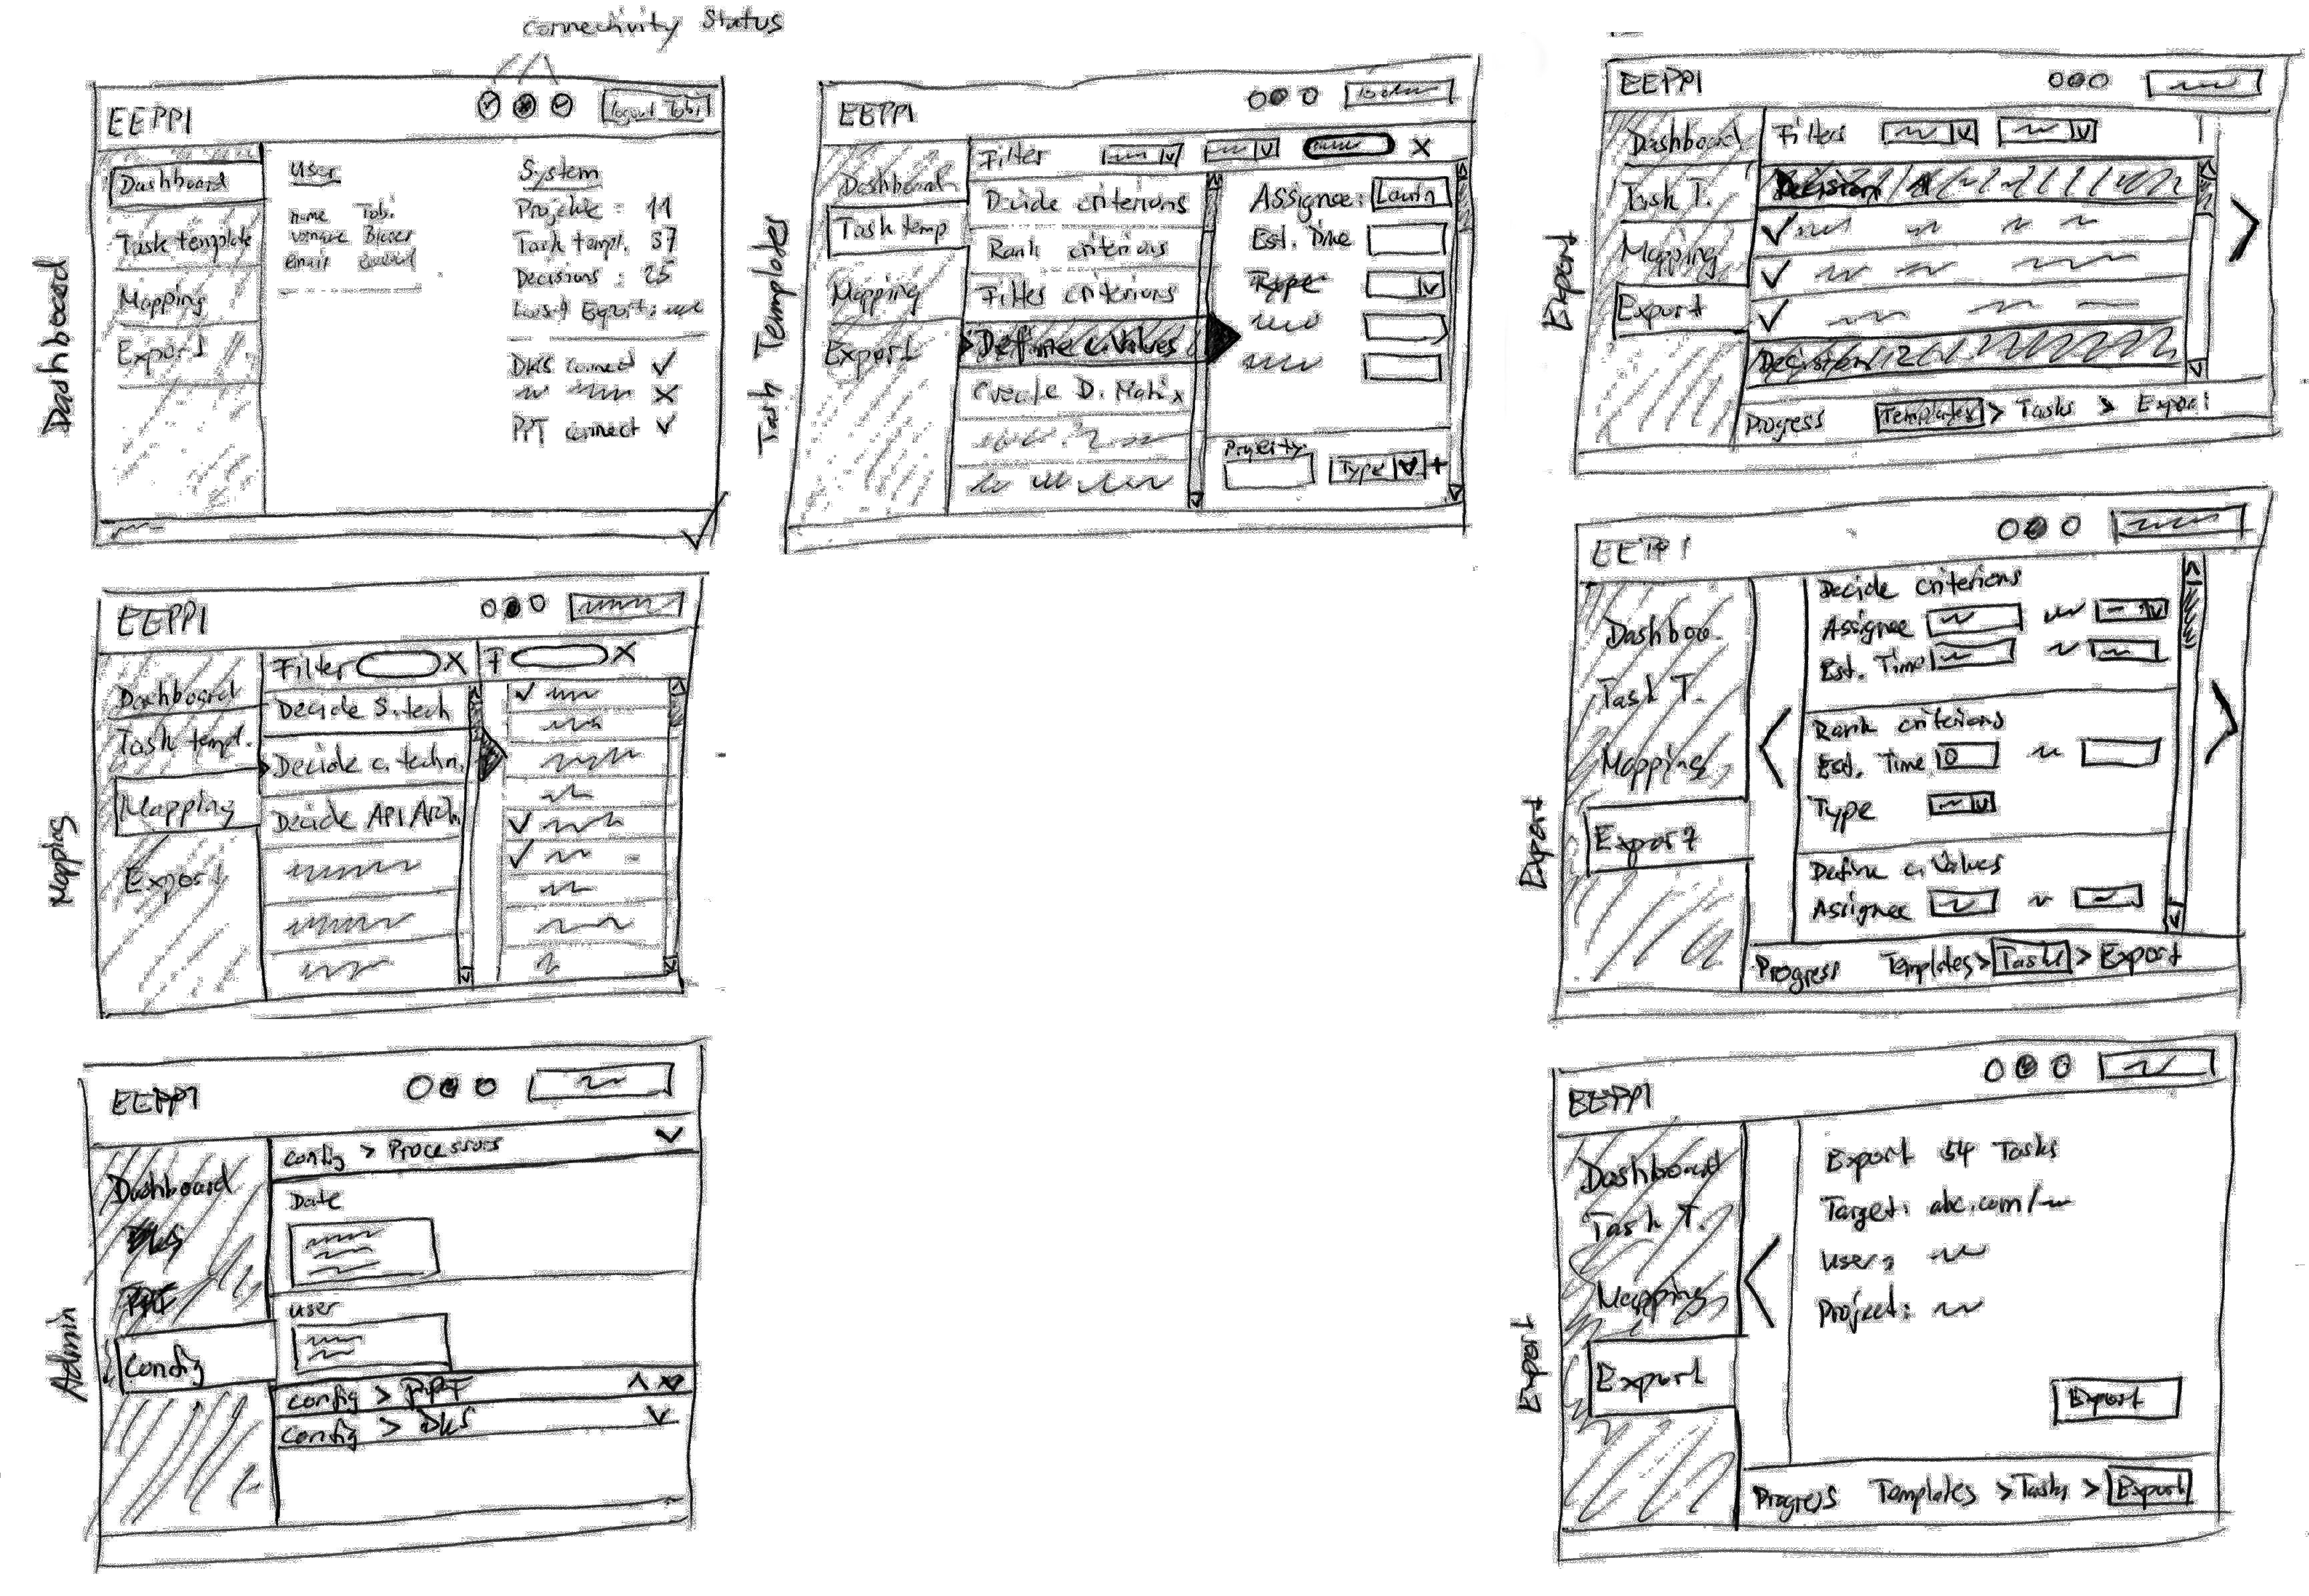
\includegraphics[width=\linewidth]{interfacesAndProtocols/media/img/wireframesTobias1.jpg}
			\centering
			\caption{Wireframes Tobias}
			\label{fig:wireframesTobias1}
		\end{figure}
		
		\begin{figure}[H]
			\begin{minipage}[b]{0.5\linewidth}
				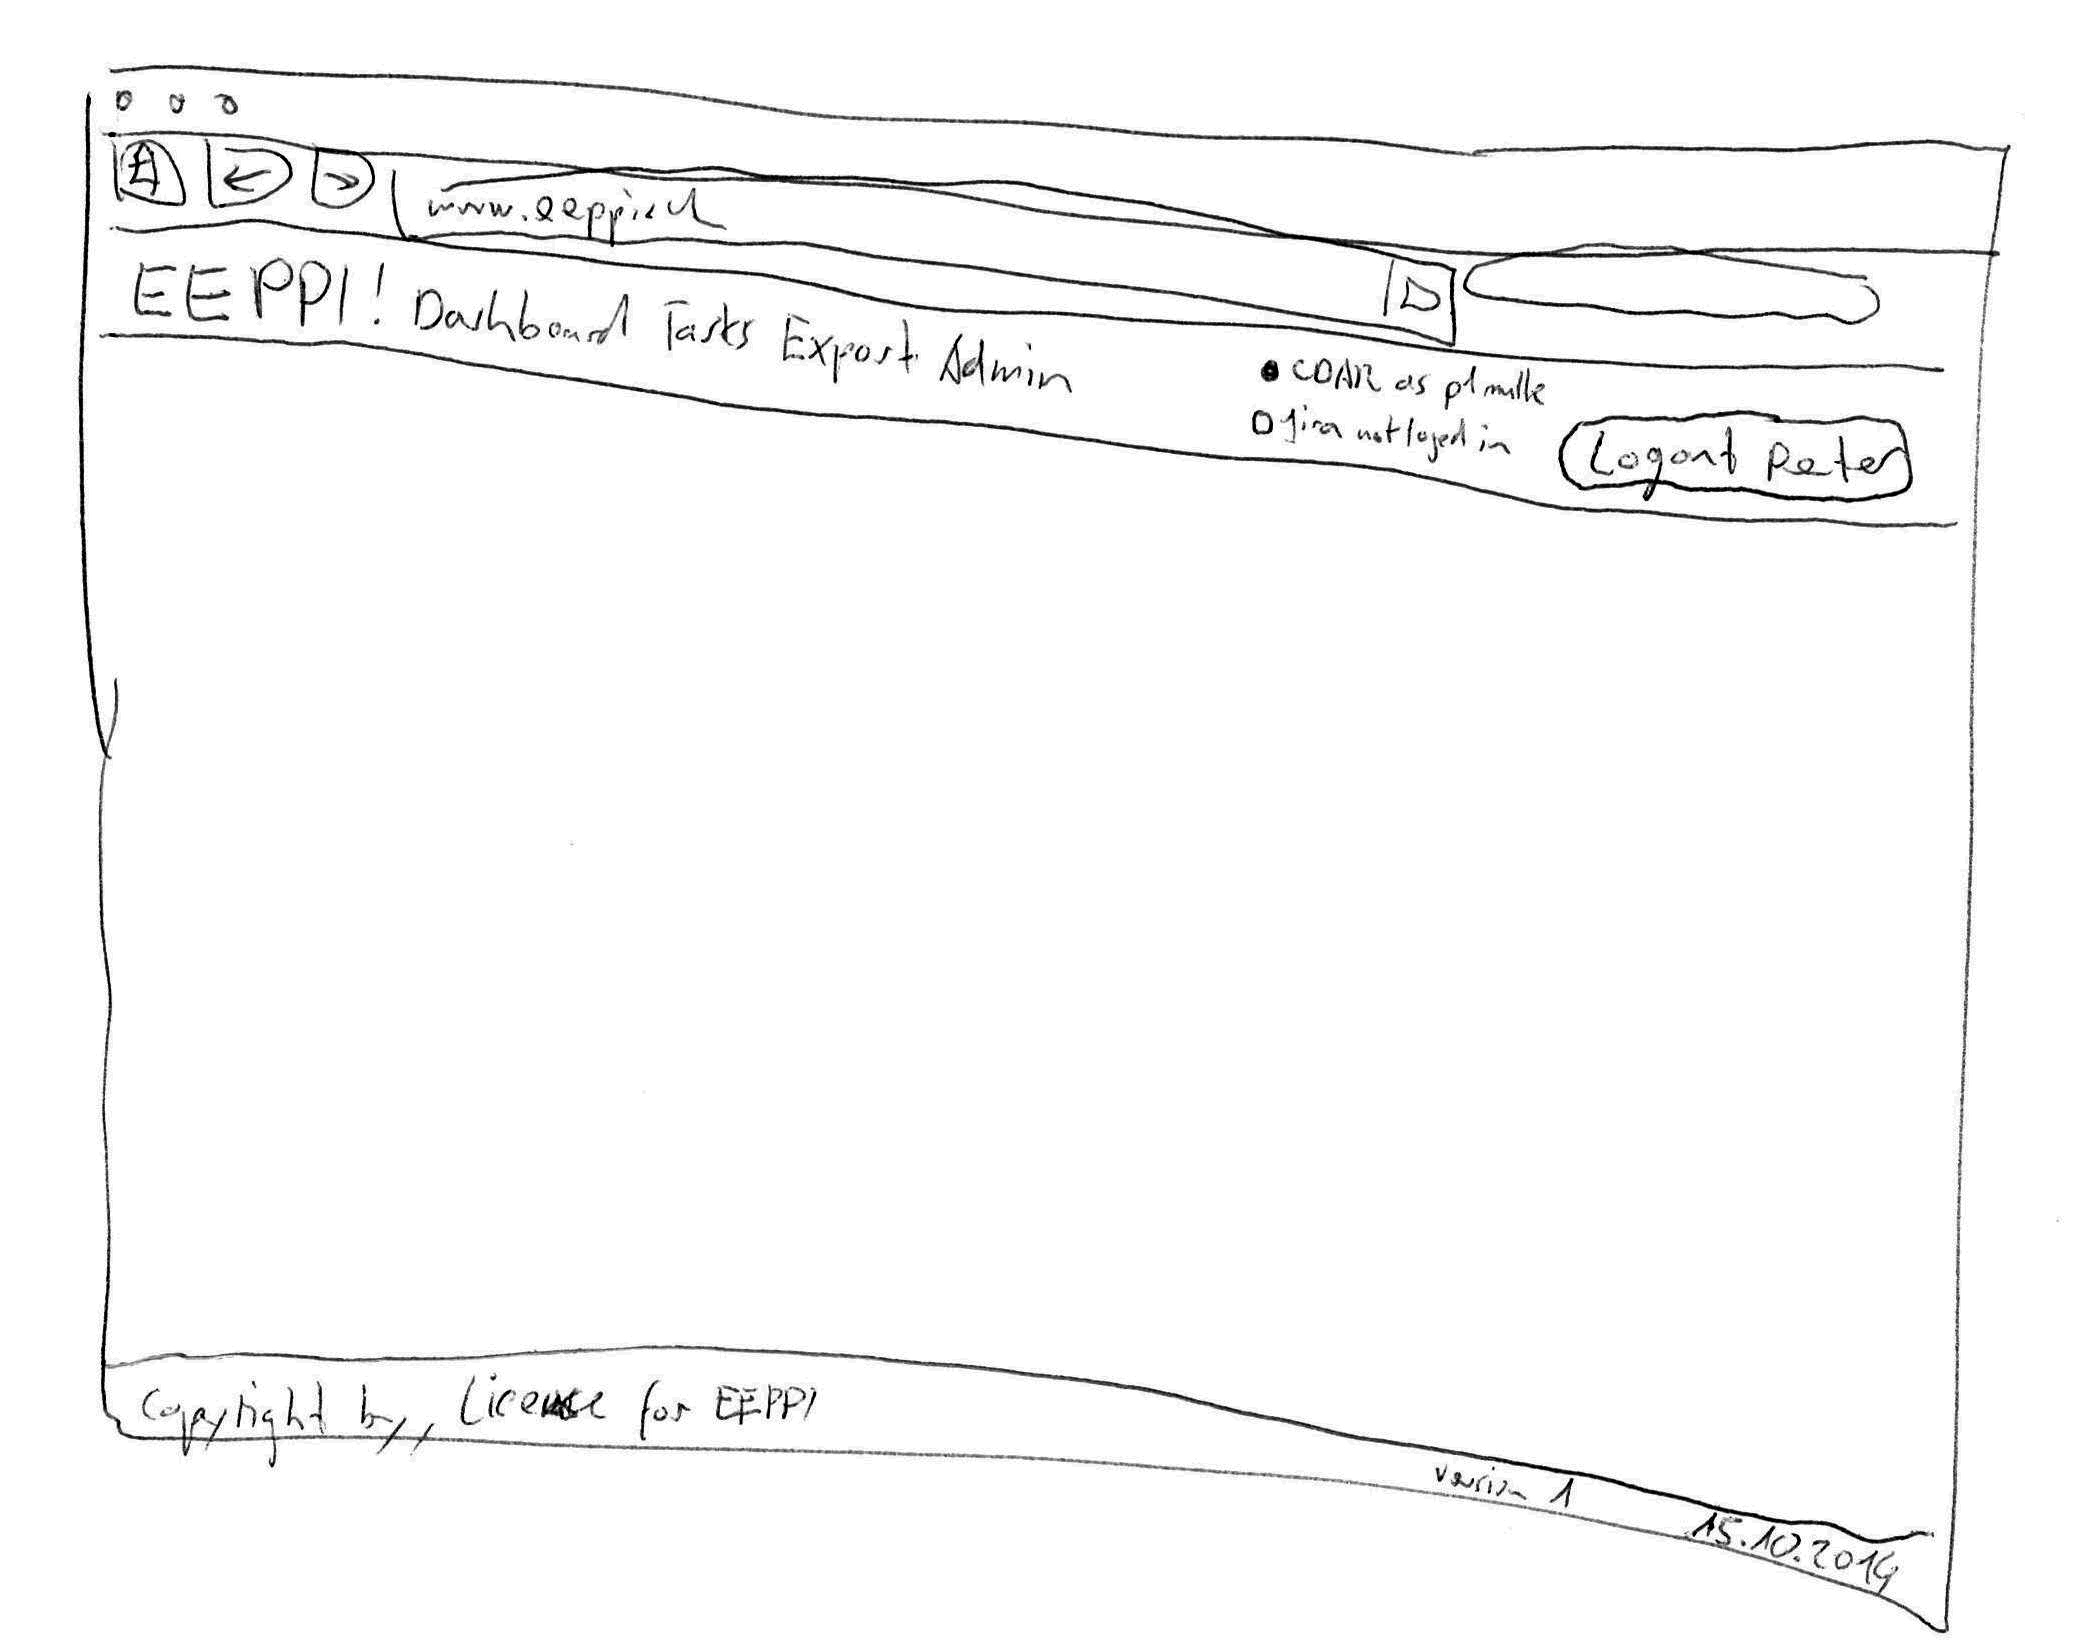
\includegraphics[width=\linewidth]{interfacesAndProtocols/media/img/wireframesLaurin1.jpg}
			\end{minipage}
			\begin{minipage}[b]{0.5\linewidth}	
				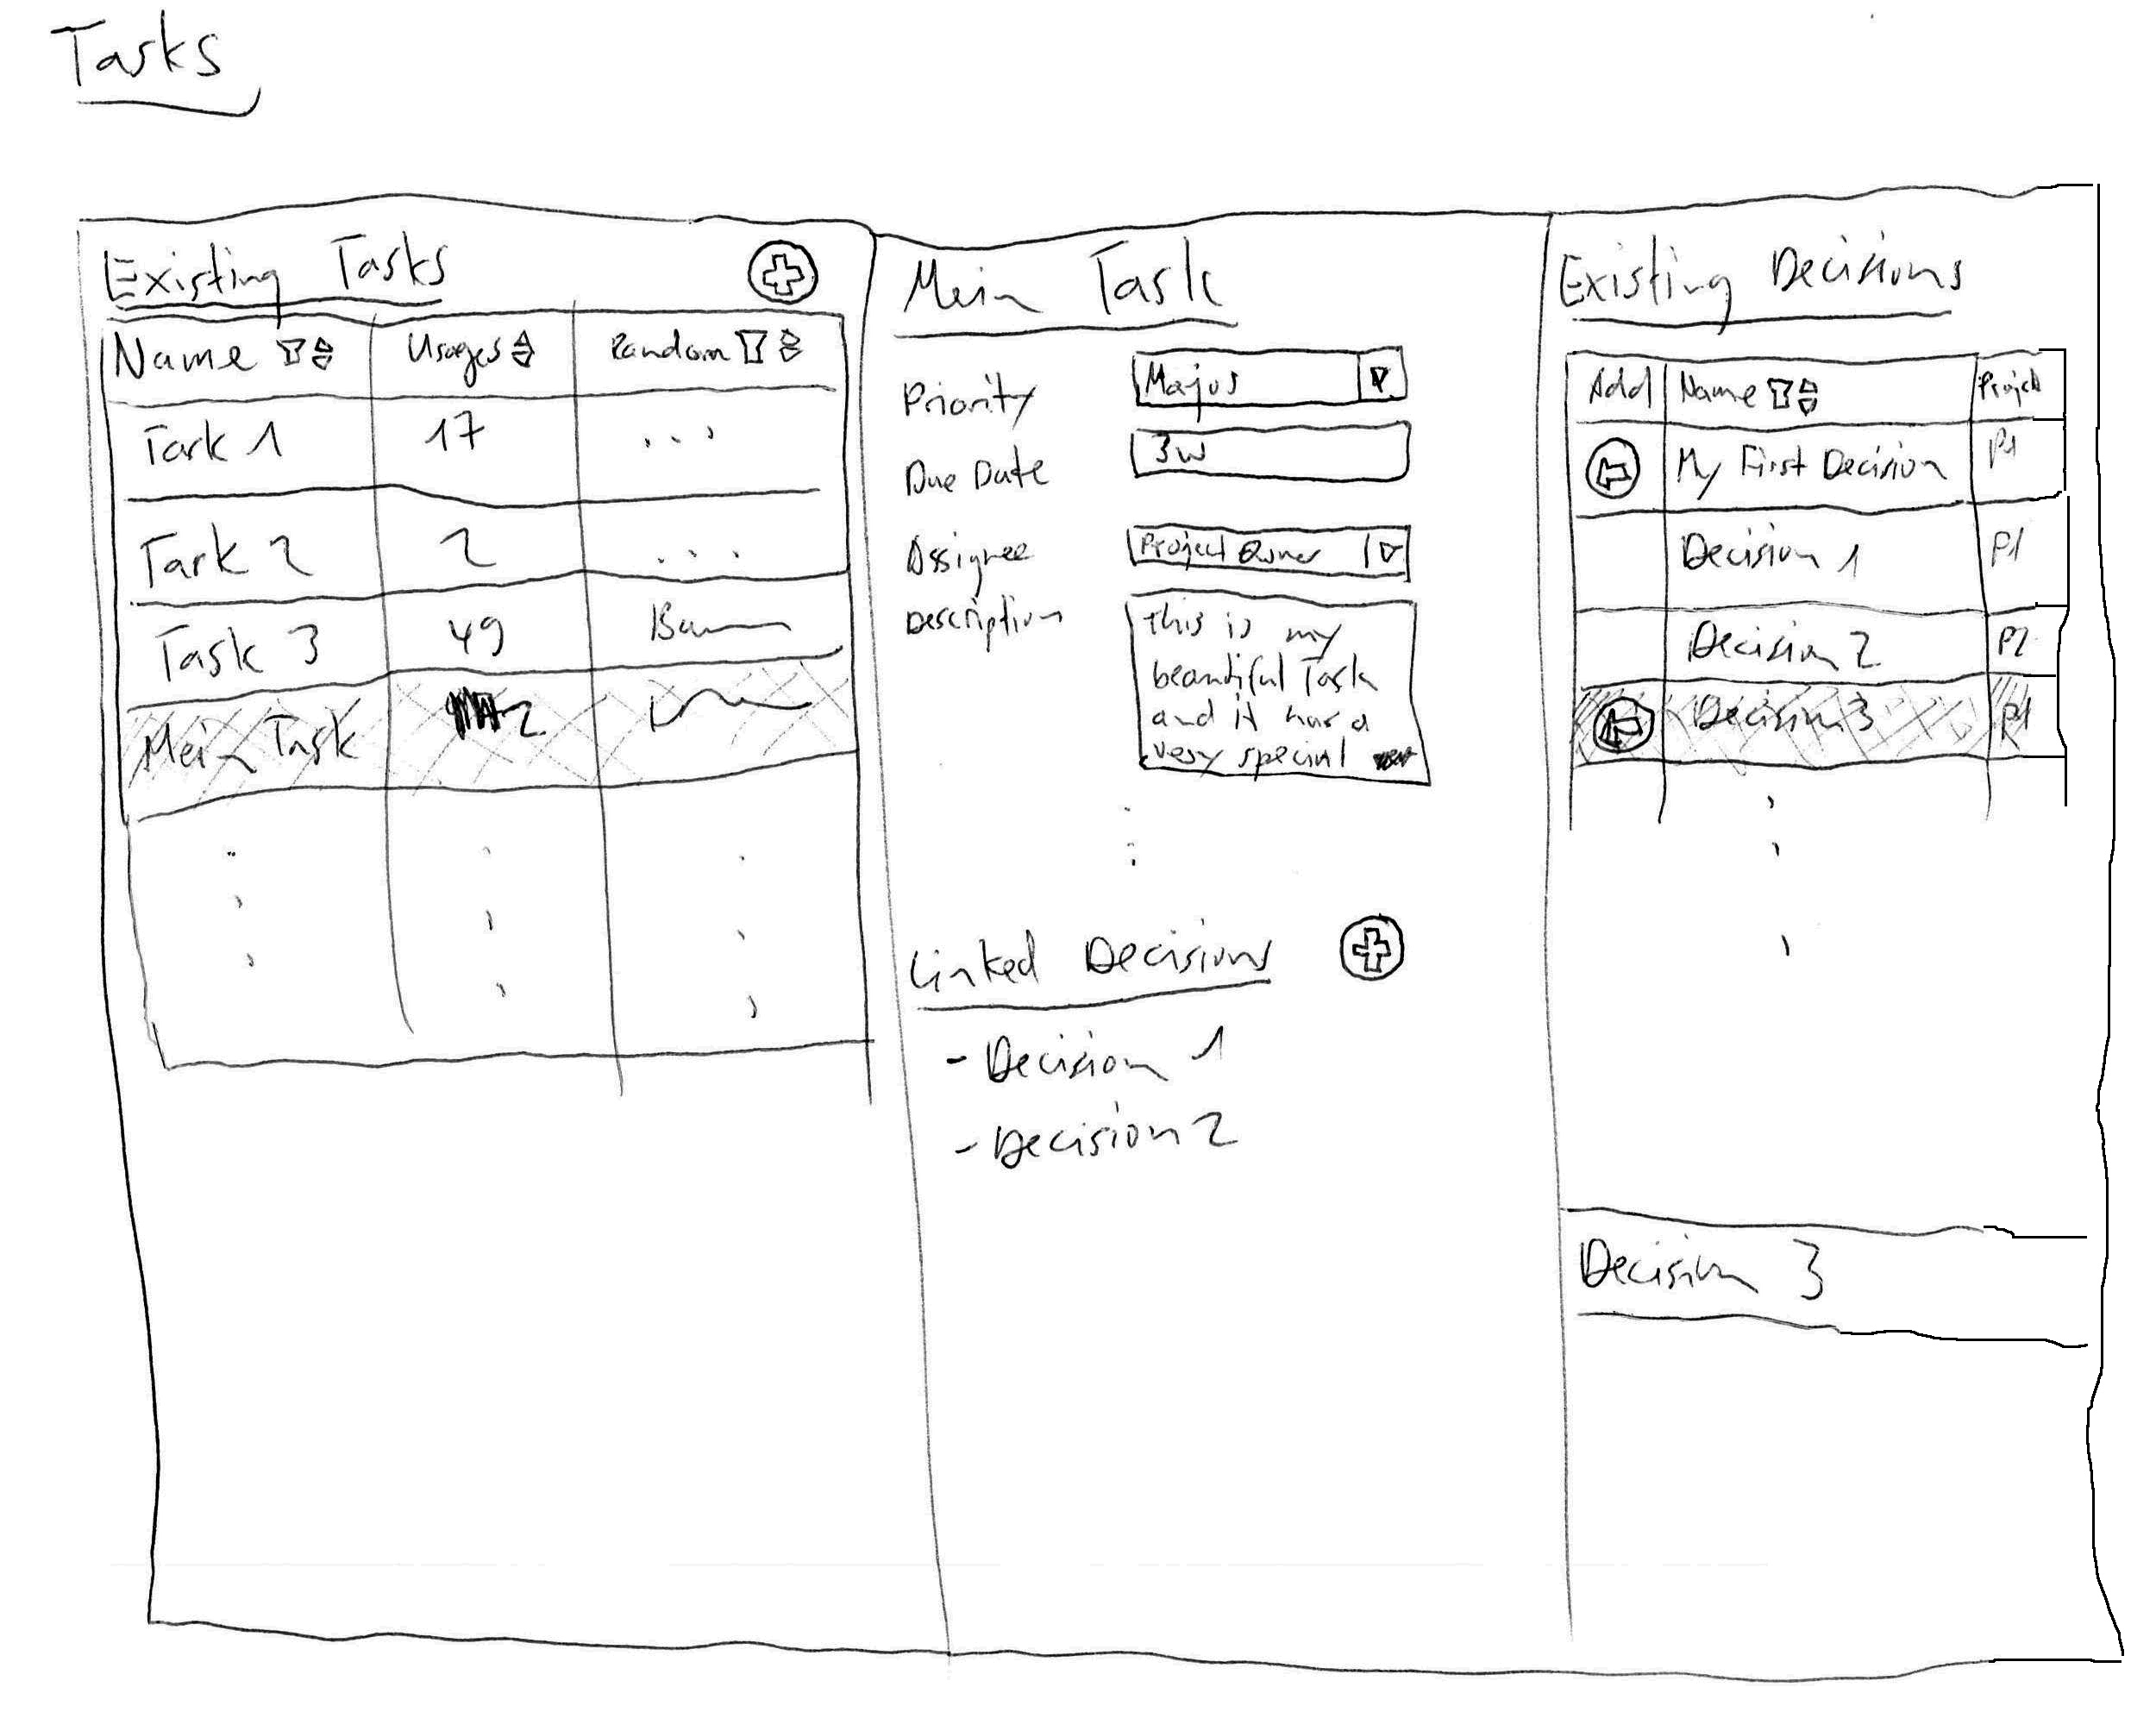
\includegraphics[width=\linewidth]{interfacesAndProtocols/media/img/wireframesLaurin2.jpg}
			\end{minipage}
		\end{figure}
		
		\begin{figure}[H]
			\begin{minipage}[b]{\linewidth}		
				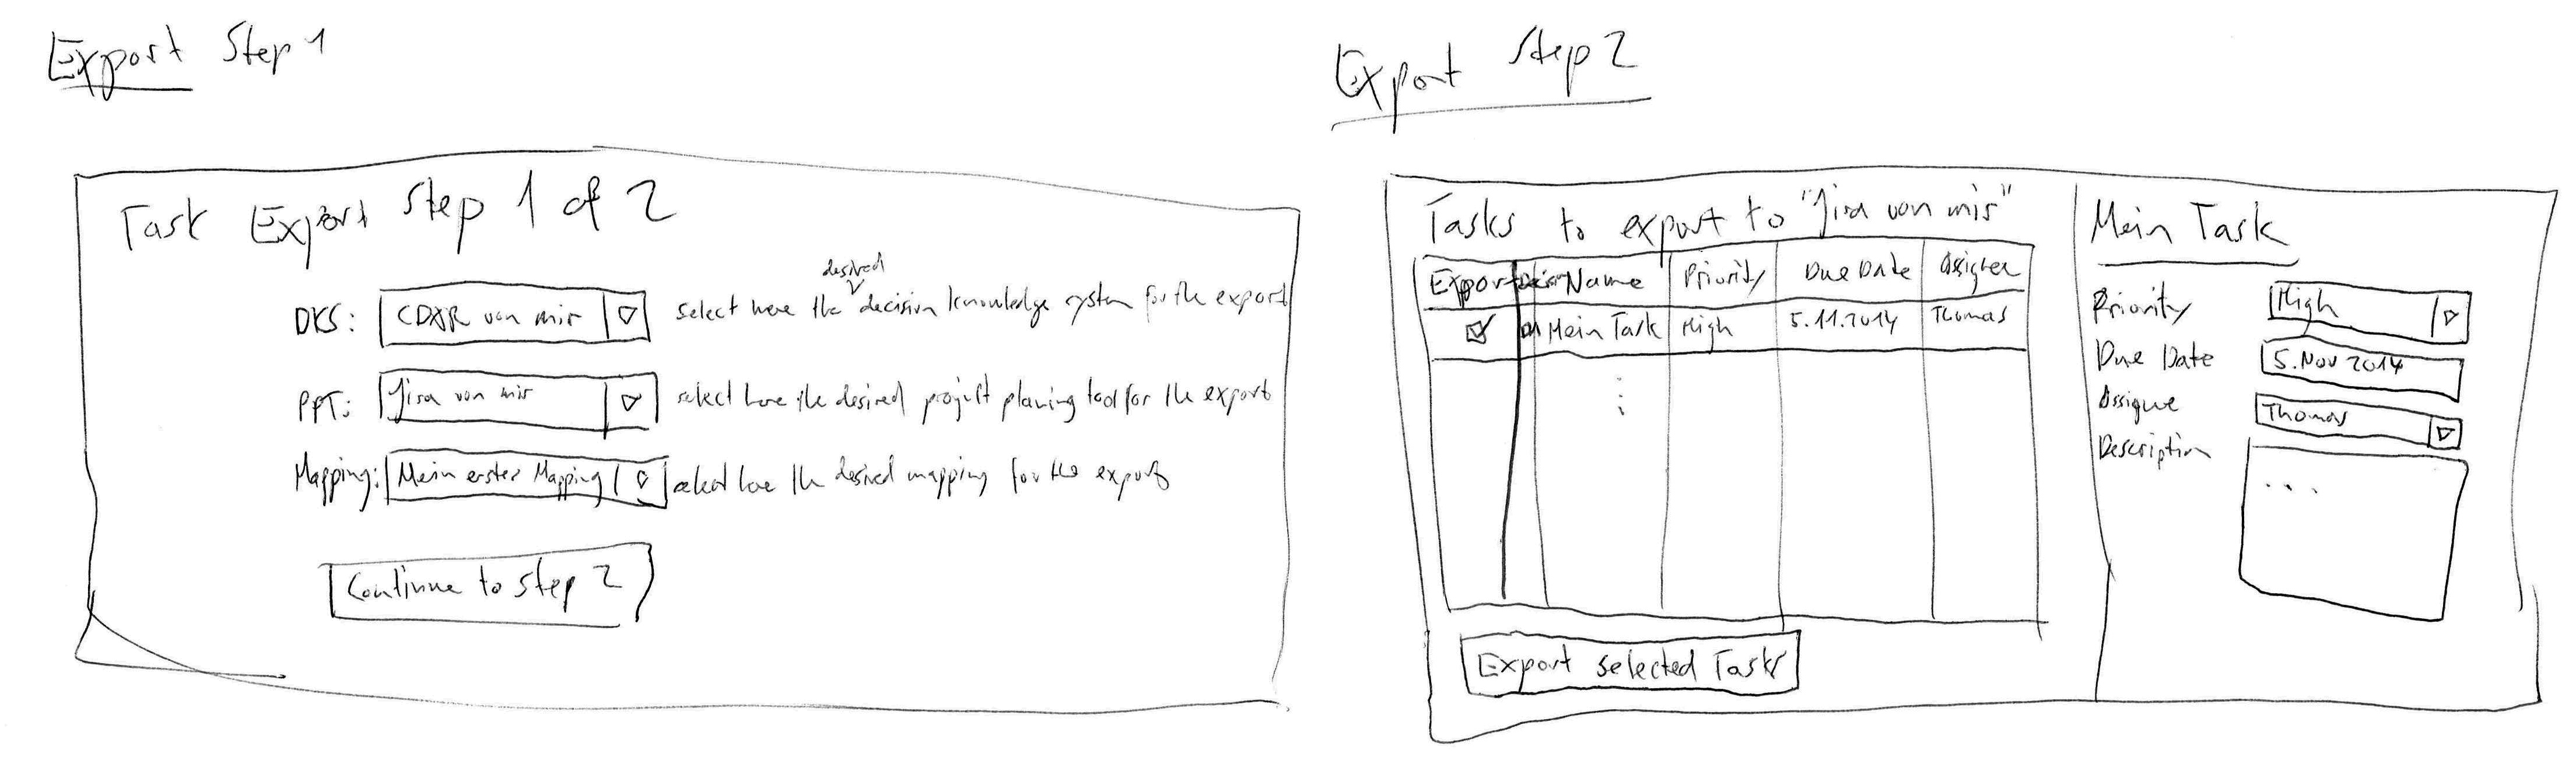
\includegraphics[width=\linewidth]{interfacesAndProtocols/media/img/wireframesLaurin3.jpg}
			\end{minipage}			
			\centering
			\caption{Wireframes Laurin}
			\label{fig:wireframesLaurin}
		\end{figure}
		
		Anschliessend wurden diese Entwürfe gemeinsam gesichtet, 
		Wireframes aussortiert oder ausgewählt und Ideen zu neuen Wireframes kombiniert.
		
		\begin{figure}[H]
			\begin{minipage}[b]{0.5\linewidth}
				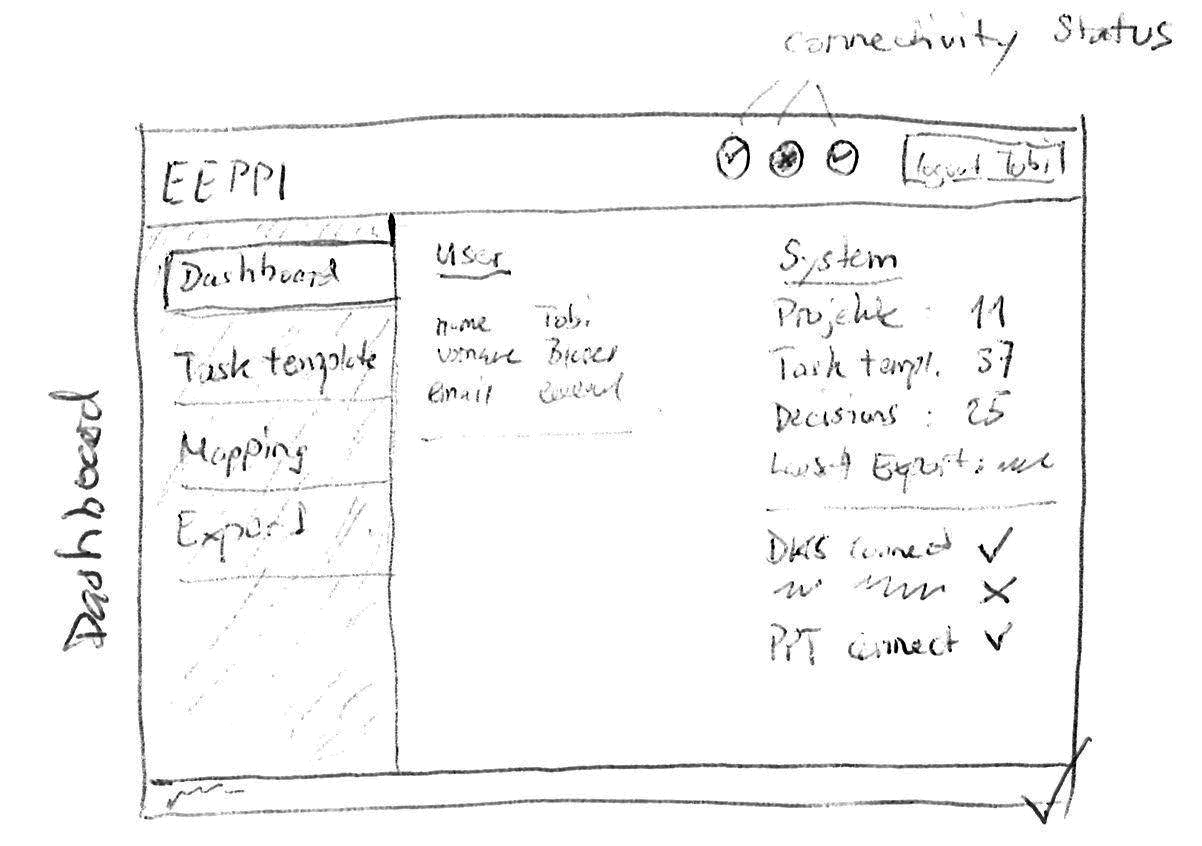
\includegraphics[width=\linewidth]{interfacesAndProtocols/media/img/dashboard.jpg}
			\end{minipage}
			\begin{minipage}[b]{0.5\linewidth}	
				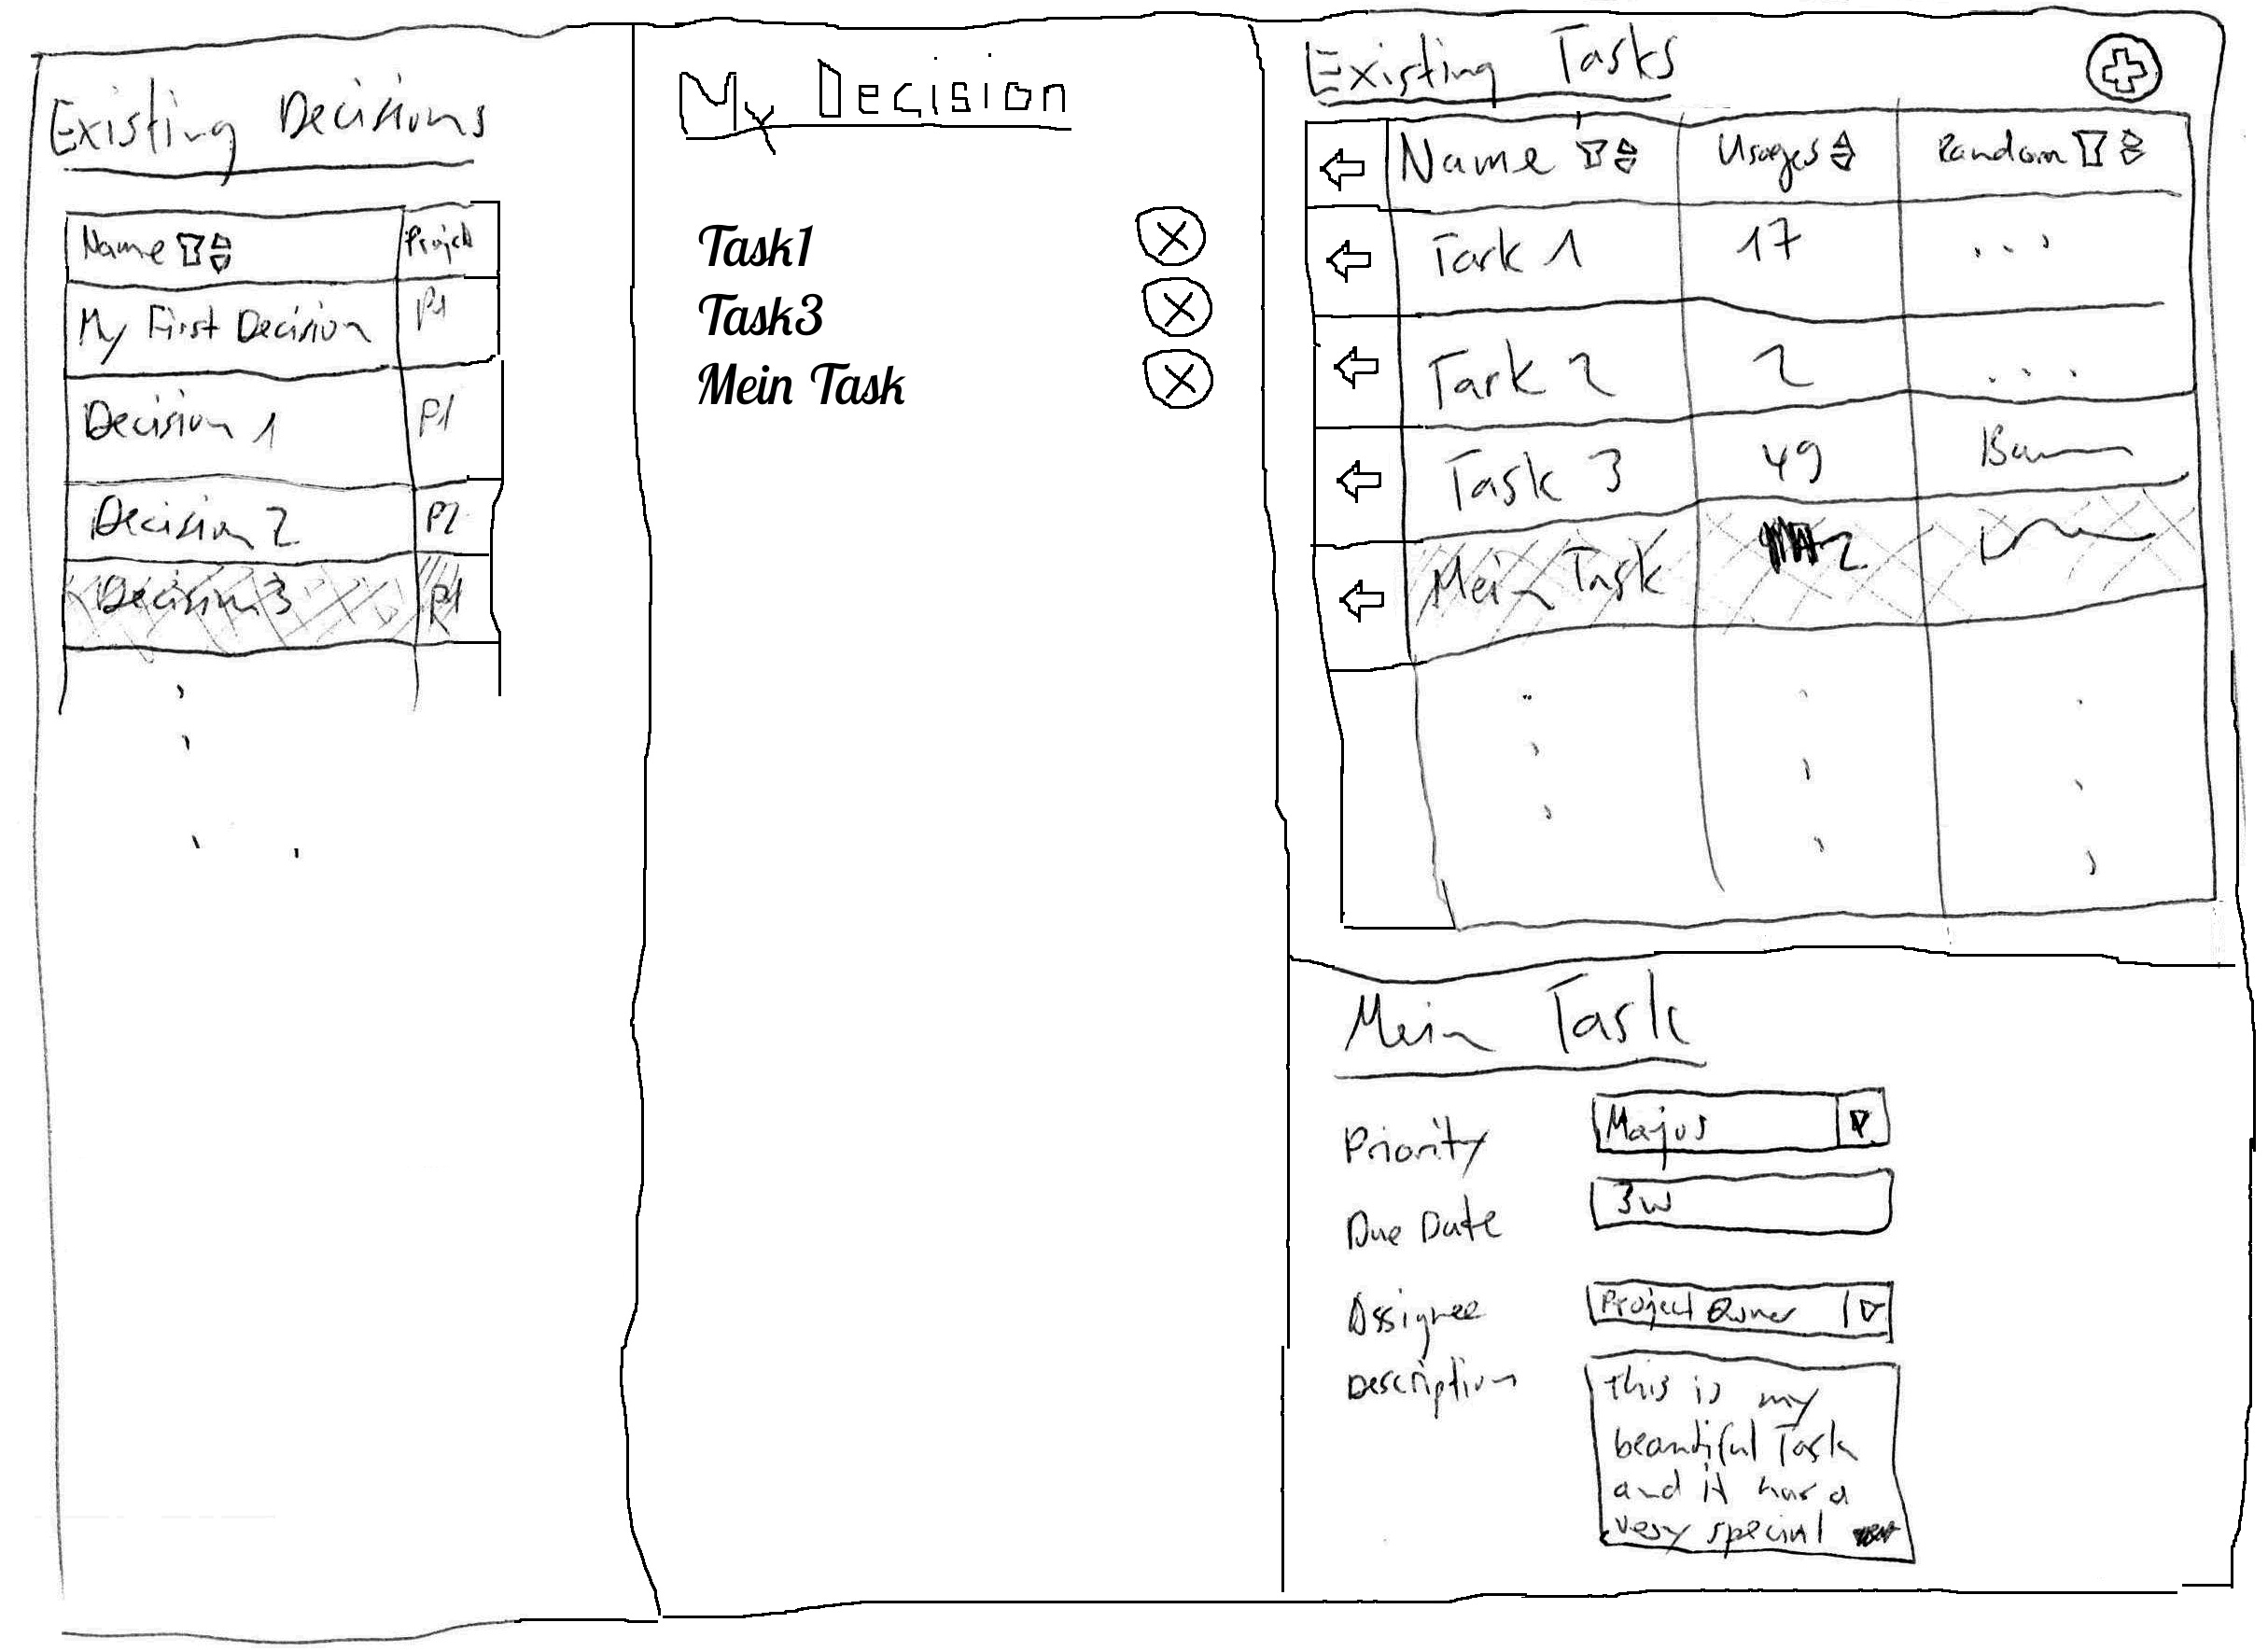
\includegraphics[width=\linewidth]{interfacesAndProtocols/media/img/tasks.jpg}
			\end{minipage}
			\caption{Dashboard \& Tasks}
			\label{fig:dashboardAndTasks}
		\end{figure}
		
		Für den Taskexport fiel die Entscheidung auf einen Assistent mit drei Schritten:
		\begin{enumerate}
			\item Auswählen von Projekt und \dks\ sowie des Mapping sets
			\item Bearbeiten der zu exportierenden Tasks, entfernen von nicht gewünschten
			\item Auswahl des \ppt, exportieren sowie Übersicht über den Status eines laufenden Exports
		\end{enumerate}
		
		Eine Progressbar im unteren Bereich soll dem Benutzer jederzeit anzeigen, bei welchem Schritt er sich befindet.
		
		\begin{figure}[H]
			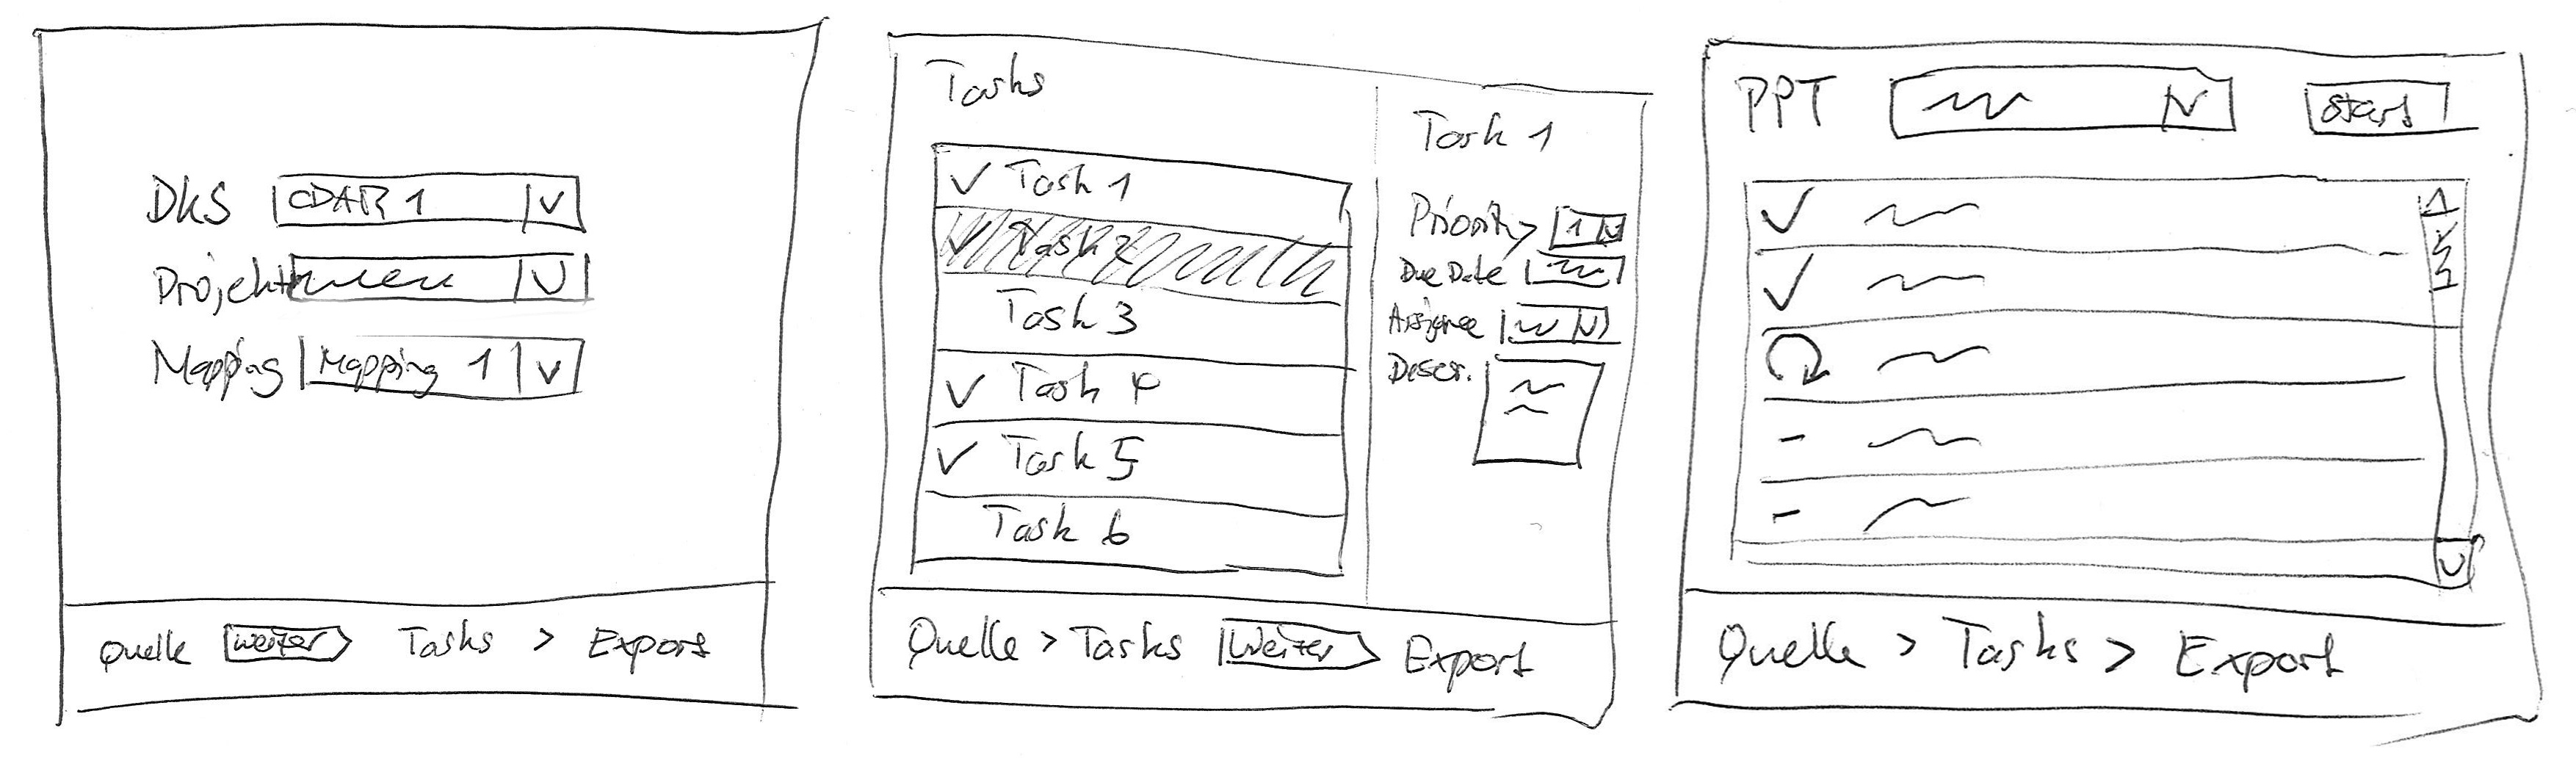
\includegraphics[width=\linewidth]{interfacesAndProtocols/media/img/exportWorkflow.jpg}
			\caption{Export Assistent}
			\label{fig:exportAssistent}
		\end{figure}	
		
		Der Benutzer kann nur weitergehen, nicht jedoch zurück, da dies durch den Umstand, 
		dass aus Task-Vorlagen Tasks generiert werden, 
		zu Datenverlust führen könnte.
		
		\begin{figure}[H]
			\centering
			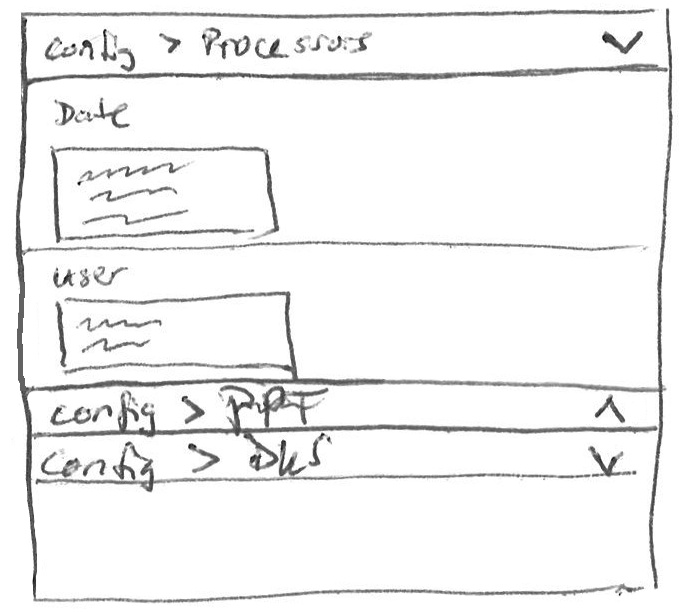
\includegraphics[width=0.3\linewidth]{interfacesAndProtocols/media/img/administration.jpg}
			\caption{Export Assistent}
			\label{fig:administration}
		\end{figure}	
		
		Der Administrationsbereich setzt sich vorwiegend aus einer aufklappbaren Liste zusammen (Accordion). Dadurch wird dem Administration eine gute Übersicht und einen Schnellen Zugriff gewährleistet.
		
		Die Navigation soll entweder unterhalb des Headers oder auf der linken Seite angebracht werden. Dazu soll während der Umsetzung überprüft werden, ob auf der Linken Seite genügend Platz vorhanden ist, wenn die Mapping Ansicht geöffnet ist.
		
		
	\section{Finales Userinterface}
	
		Anhand der Mockups und entwickelten Workflows wurde anschliessend das finale Interface umgesetzt.
		Dabei wurden iterativ Bereiche angepasst und verbessert.
		Dies war insbesondere in der Darstellung der Problems \& Task Templates notwendig, 
		da wesentlich mehr Daten visualisiert werden sollten, als ursprünglich im Mockup vorgesehen.
		
		\begin{figure}[H]
			\centering
			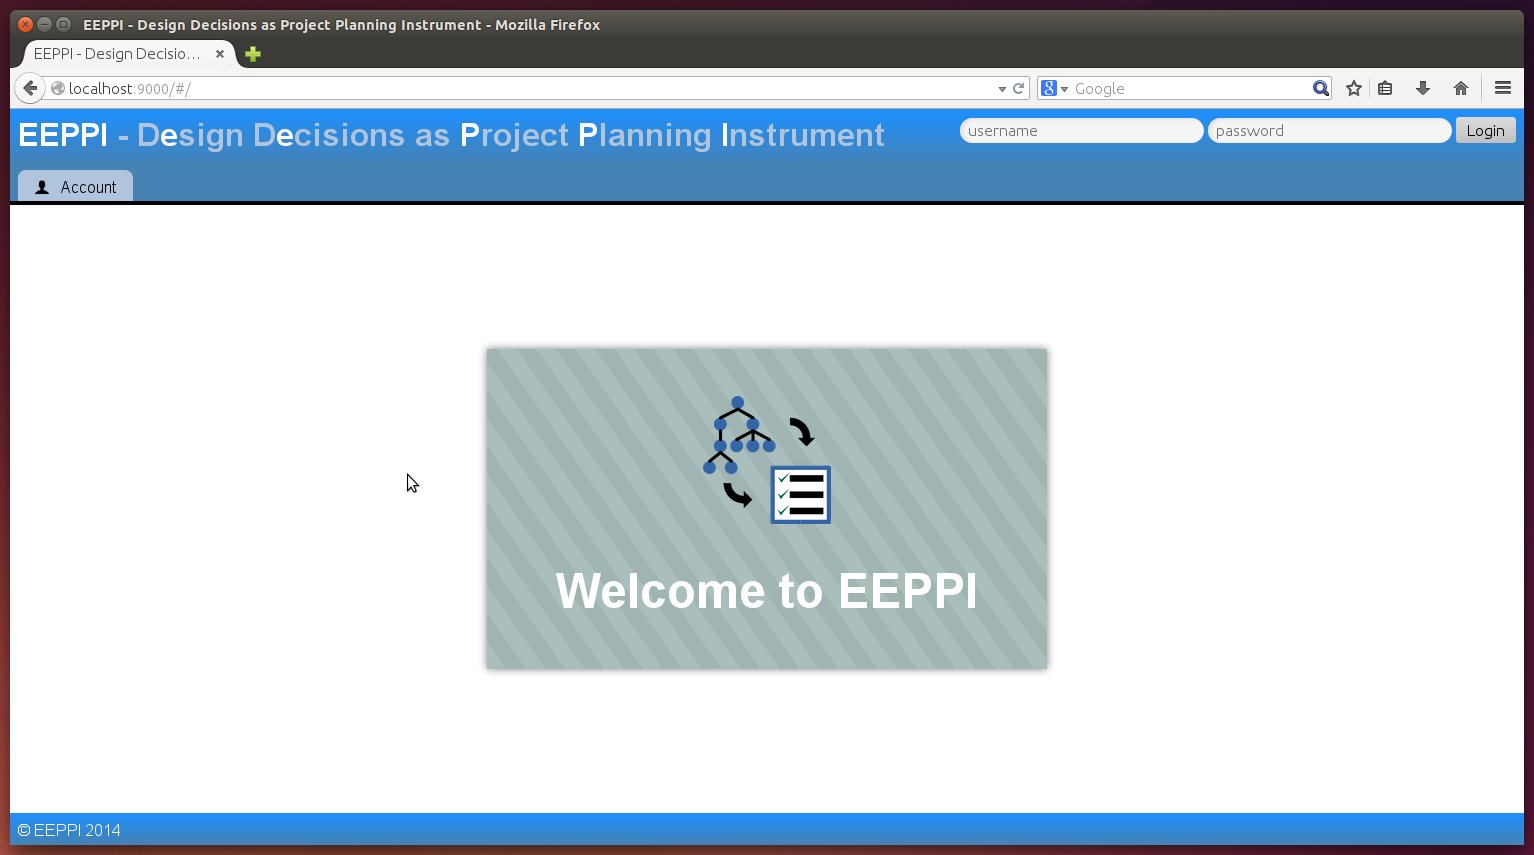
\includegraphics[width=\linewidth]{tutorial/img/eeppiHomeScreen.jpg}
			\caption{EEPPI Home Screen}
			\label{fig:eeppiHomeScreen}
		\end{figure}	
		
		Auf die Umsetzung des Dashboard wurde verzichtet, da viele der dafür notwendigen Informationen im tief priorisierten und darum nicht umgesetzten Feature "<Inform user about network and system status"> enthalten waren und entsprechend nicht verfügbar waren.
		Anstelle wurde ein einfacher Home-Screen Implementiert (siehe Abbildung\ \ref{fig:eeppiHomeScreen}).
		
		
		\begin{figure}[H]
			\centering
			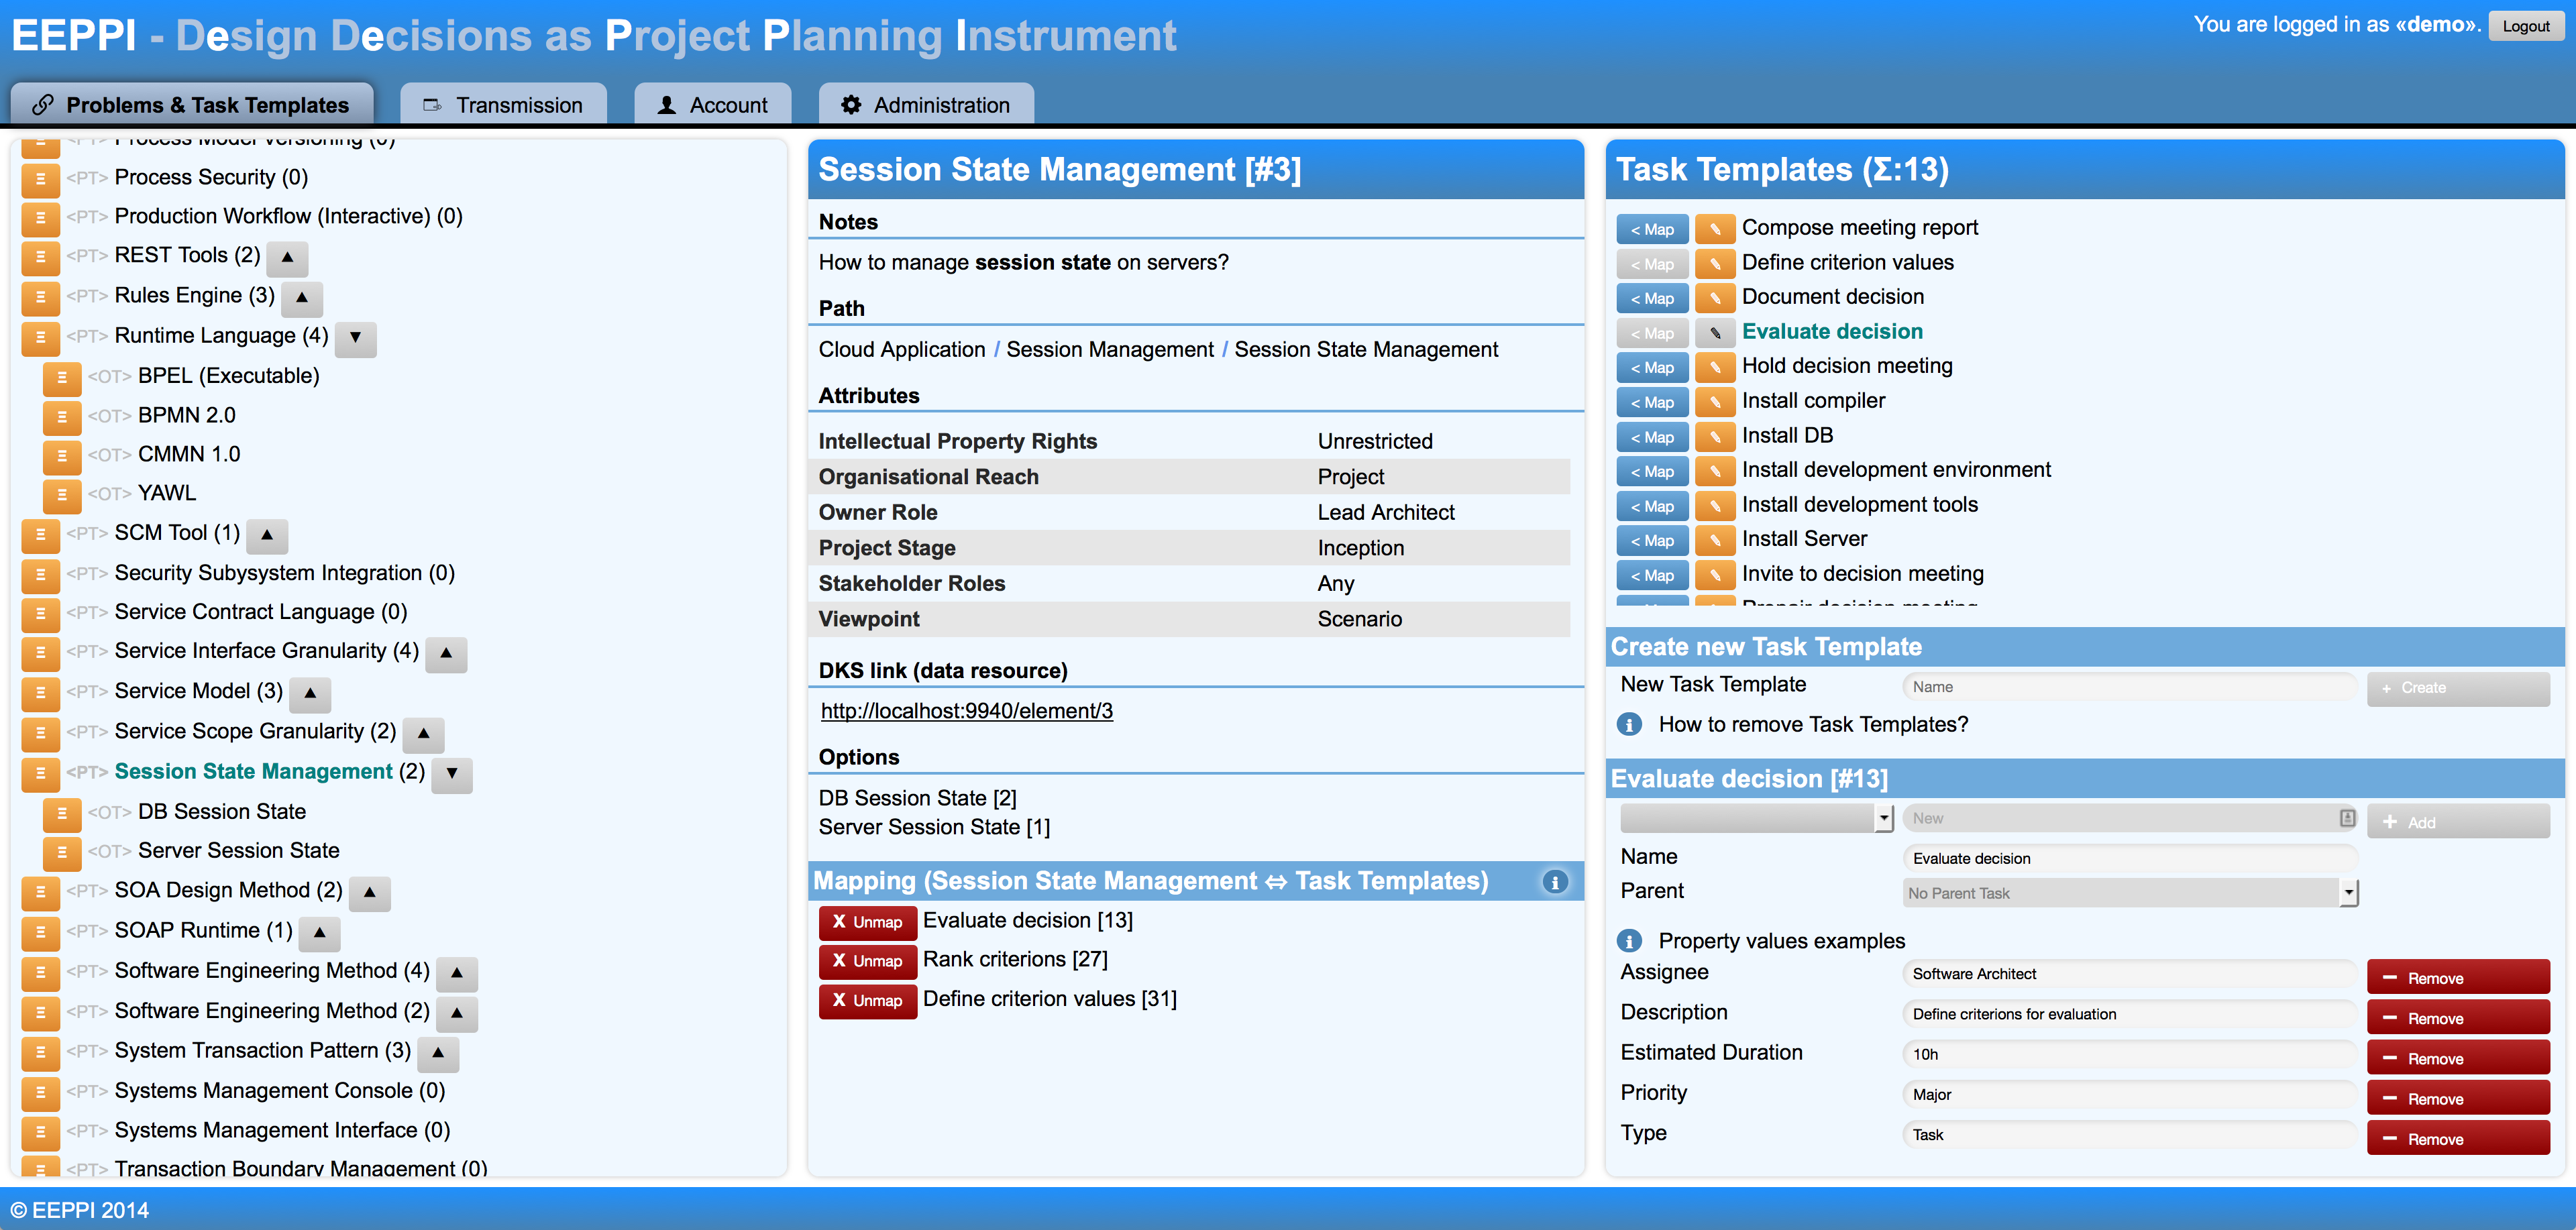
\includegraphics[width=\linewidth]{tutorial/img/eeppiDecisionsAndTaskTemplates.png}
			\caption{Problems \& Tasktemplates}
			\label{fig:eeppiDecisionsAndTaskTemplates}
		\end{figure}	
		
		Die Ansicht der verfügbaren Problems, der Tasktemplates und deren Mapping wurde nach dem Mockup umgesetzt und anschliessend noch um viele zusätzliche Informationen erweitert (Abbildung\ \ref{fig:eeppiDecisionsAndTaskTemplates}).
		So kam beispielsweise zur Detailansicht der Mappings noch eine Detailansicht des ausgewählten Problems hinzu.
		Damit kann sich der Benutzer eine besser Übersicht darüber verschaffen,
		ob er das richtige Problem mappt.
		Insbesondere bei ähnlichen Namen der Problems ist dies von Vorteil.
		In diesen Bereich wurde auch eine HTML-Unterstützung für Notes eingebaut, 
		sodass diese mit HTML-Tags ausgezeichnet werden können.
		
		
		\begin{figure}[H]
			\centering
			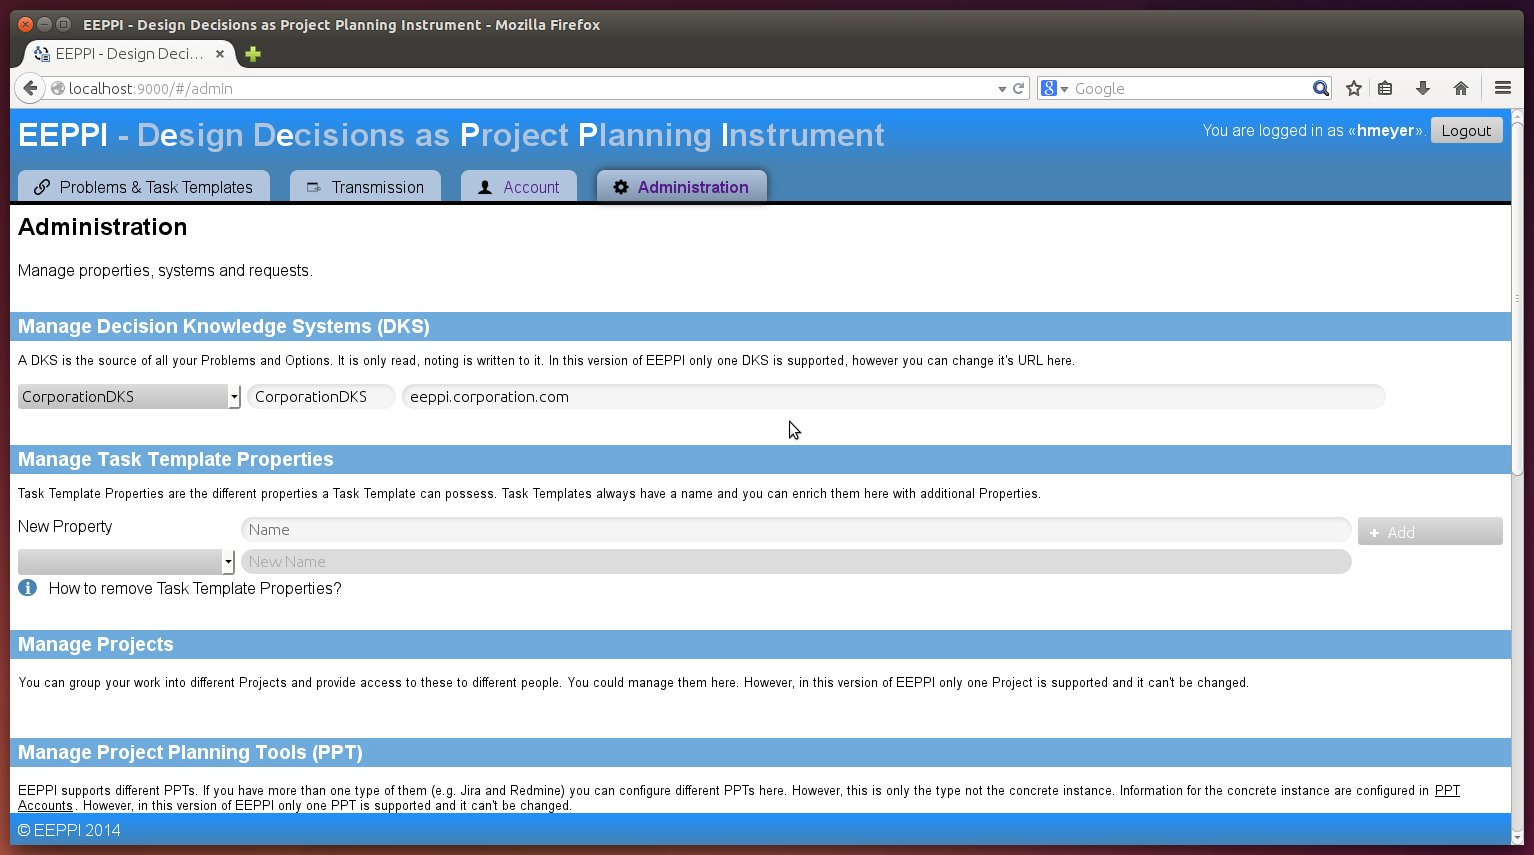
\includegraphics[width=\linewidth]{tutorial/img/administrationDKS.jpg}
			\caption{Administrationsbereich}
			\label{fig:eeppiAdministration}
		\end{figure}	
		
		Beim Administrationsbereich (Abbildung\ \ref{fig:eeppiAdministration}) haben wir uns nur sehr beschränkt an die Mockups gehalten, 
		da wir bald gemerkt haben, dass die darzustellenden Informationen nicht mit dem Mockup zusammenpassen.
		Zum Zeitpunkt als wir die Mockups erstellten, 
		war noch nicht genau klar welche Informationen in diesem Bereich untergebracht werden sollen.		
		
		
		\begin{figure}[H]
			\centering
			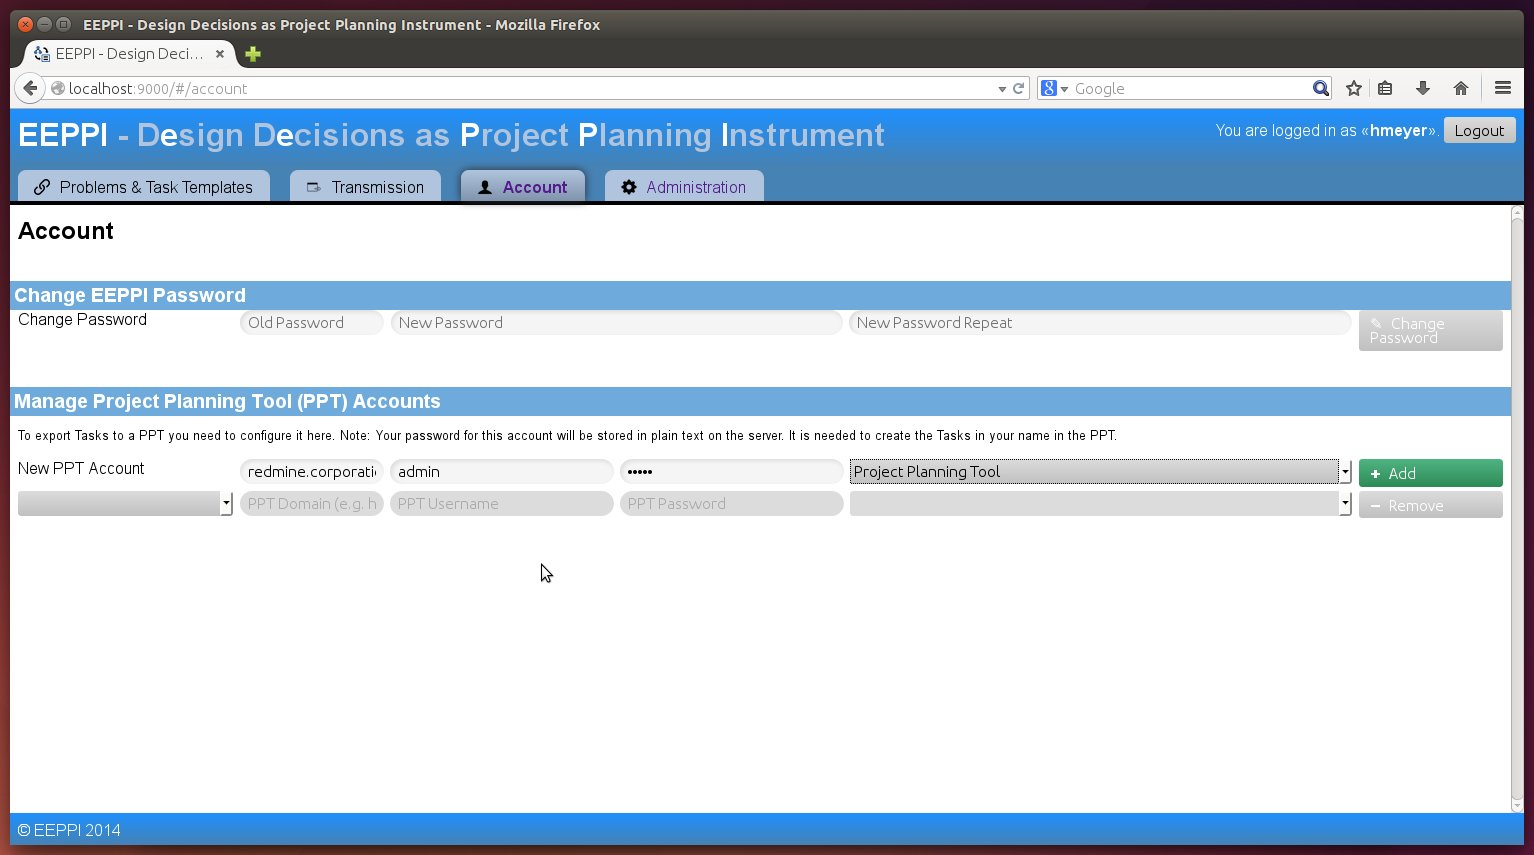
\includegraphics[width=\linewidth]{tutorial/img/accountPPTAccount.jpg}
			\caption{Accountverwaltung}
			\label{fig:eeppiAccountManagement}
		\end{figure}	
		
		Für den Accountverwaltungsbereich (Abbildung\ \ref{fig:eeppiAccountManagement}) gab es keine Mockups, da zum damaligen Zeitpunkt noch Unklarheit über das Usermanagement bestand.
		Entsprechend wurde dieses analog der Administration gestaltet.
		
			
		\begin{figure}[H]
			\centering
			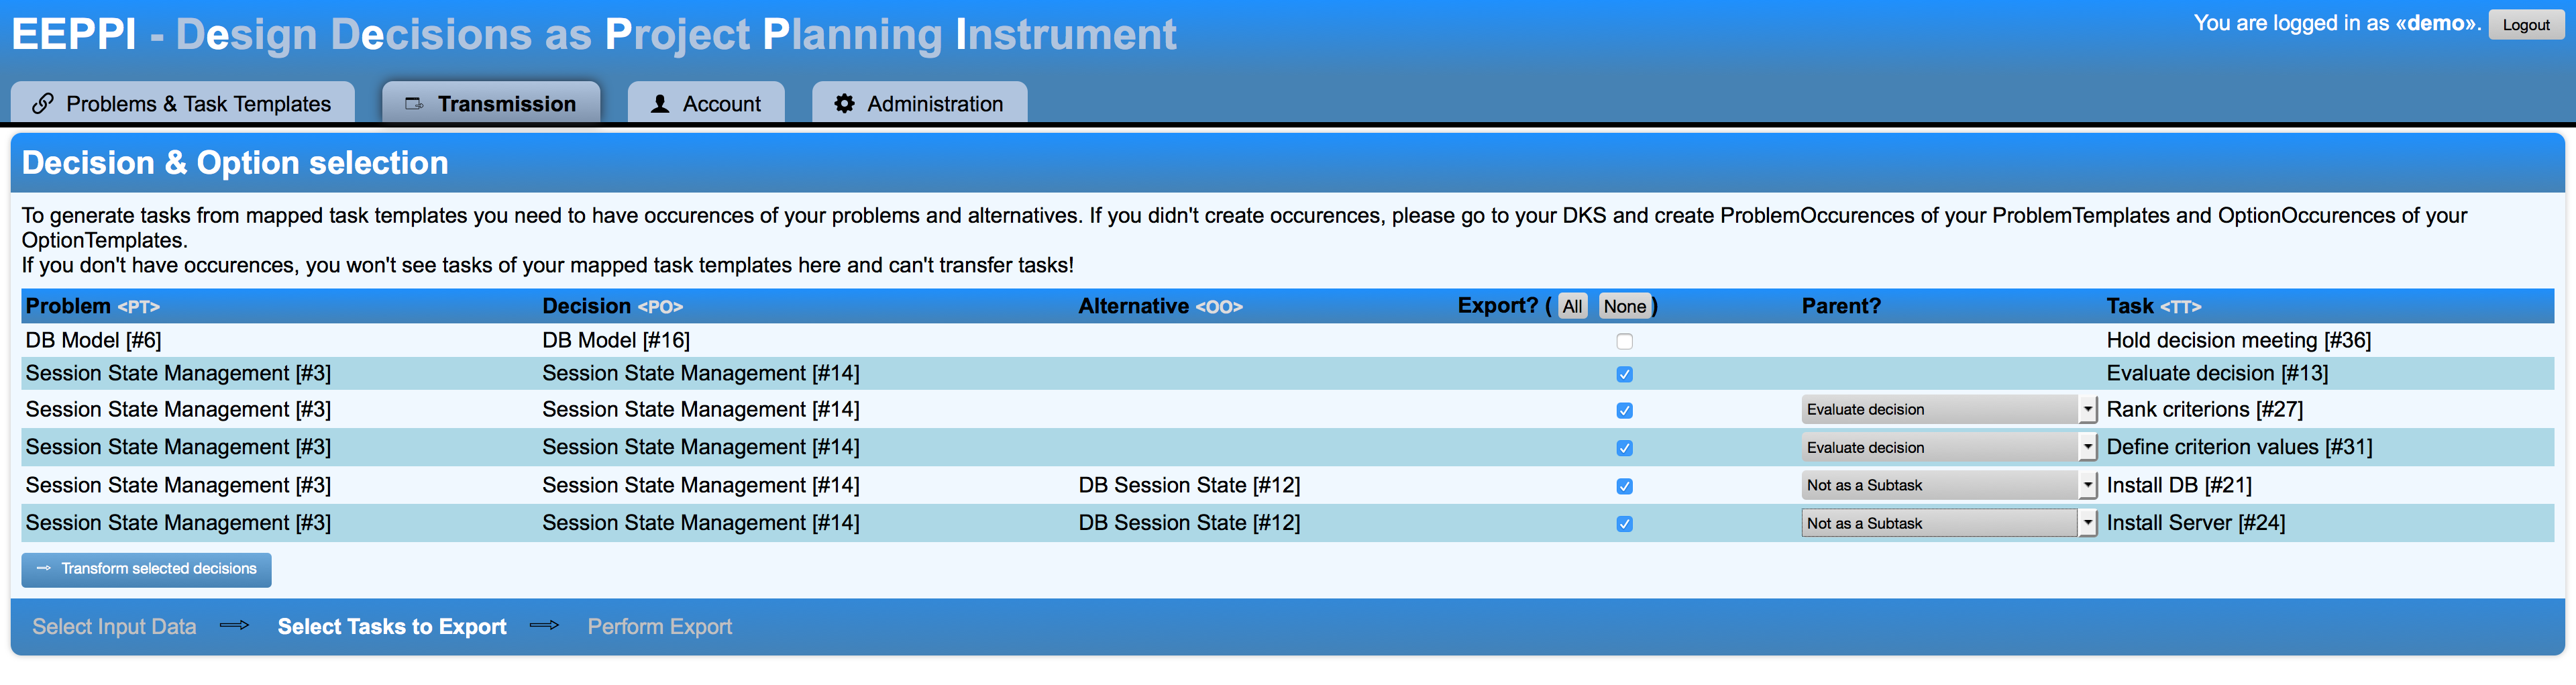
\includegraphics[width=\linewidth]{tutorial/img/transmit2.png}
			\caption{Übertragen von Tasks an ein \ppt}
			\label{fig:eeppiTransmissionScreen}
		\end{figure}	
		
		Im Übertragungsbereich (Abbildung\ \ref{fig:eeppiTransmissionScreen}) ist gegenüber den Mockups die Editierfunktion für zu exportierende Tasks entfallen,
		dieses Feature wurde vom Betreuer, als Ansprechpartner der Kundengruppe, mit niedriger Priorität eingestuft.
